\chapter{Dagens pasientsignalsystem ved St. Olavs Hospital}
\label{appendix_dagenssystem}
Dette tillegget inneholder en beskrivelse av dagens pasientsignalsystem ved St.Olavs Hospital. Tekst og bilder er hentet fra opplæringsdokumenter og brukermanualer gitt ved St. Olavs Hospital, tilgjengelig på deres hjemmesider \cite{BrukerveiledningforPasientsignal, BrukermanualforPasientsignalogPasientsignalapplikasjon, BrukerveiledningforTradlostelefon}

\section{Dagens pasientsignalsystem}
Et signal utløses fra blandt annet sengerom, fellesrom, stuer og toalett, for å tilkalle/alarmere pleiepersonell. Det skilles mellom to typer signaler: (1) Pasientsignal, som utløses av pasienten selv, og (2) hasteanrop, som utløses av pleiepersonell ved behov for umiddelbar assistanse. Pasientsignalsystemet er sammensatt av to integrerte systemer, et fast og et trådløst. 

\subsection{Pasientsignalanlegget - det faste systemet}
Det faste systemet, også refererert til som pasientsignalanlegget, består av fastmonterte paneler med trekksnorer og/eller trykknapper. Disse er illustrert i figur \ref{pasientsignalanlegget}.

\begin{figure}[H]
        \centering
        \begin{subfigure}[b]{0.3\textwidth}
        		\centering
                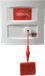
\includegraphics[scale=0.7]{anropspanel.png}
                \caption{Anropspanel}
                \label{anropspanel}
        \end{subfigure}%
        \begin{subfigure}[b]{0.3\textwidth}
        		\centering
                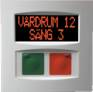
\includegraphics[scale=1.5]{rompanel.jpg}
                \caption{Rompanel}
                \label{rompanel}
        \end{subfigure}
        \begin{subfigure}[b]{0.3\textwidth}
        		\centering
                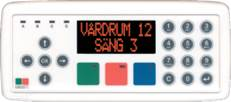
\includegraphics[scale=1]{vaktromsapparat.jpg}
                \caption{Vaktromsapparat}
                \label{vaktromsapparat}
        \end{subfigure}
        \caption{Pasientsignalanlegget}
        \label{pasientsignalanlegget}
\end{figure}

\noindent
\subsubsection{Anropspanelet}
Det finnes to typer anropspanel, et for våtrom og et for vanlig rom. I vanlige sengerom er anropspanelet plassert ved sengen, og har en trykknapp med lysdiode og en trekksnor.
Trykknappen utløser et hasteanrop, mens trekksnoren utløser et pasientsignal.

\subsubsection{Rompanelet}
Rompanelet er plassert ved døren til hvert av sengerommene på tunet. Det har et display, og en grønn og en rød trykknapp med hver sin lysdiode. Grønn knapp trykkes for å markere pleiepersonells tilstedeværelse eller for å avstille et signal. Rød knapp trykkes for å utløse pasientsignal, eller et hasteanrop dersom tilstedemarkering er aktivert. Rød knapp kan også holdes inne i 2 sekunder for å utløse hasteanrop, dersom tilstedemarkering ikke er aktivert. 

\subsubsection{Vaktromsapparatet}
Vaktromsapparatet er sentralt plassert i det åpne landskapet på sengetunet. Det består av et display og flere tall- og tegntaster. Displayet indikerer stedangivelse for et pasientsignal, hasteanrop og tilstedemarkerte rom. Pasientsignaler og hasteanrop er signalisert med rød tekst, mens tilstedemarkering er vist ved grønn tekst. Tall- og tegntastene brukes for å programmere apparatet.

\subsection{Det trådløse systemet}
Pasientsignalanlegget er videre tilkoblet det trådløse systemet, som består av følgende IKT-komponenter: pasientsignalapplikasjon, trådløs telefonenhet og pasientterminal, illustrert i figur \ref{pasientapplikasjon}, \ref{telefonenhet} og \ref{pasientterminal} henholdsvis.

\begin{figure}[H]
        \centering
        \begin{subfigure}[b]{0.35\textwidth}
        		\centering
                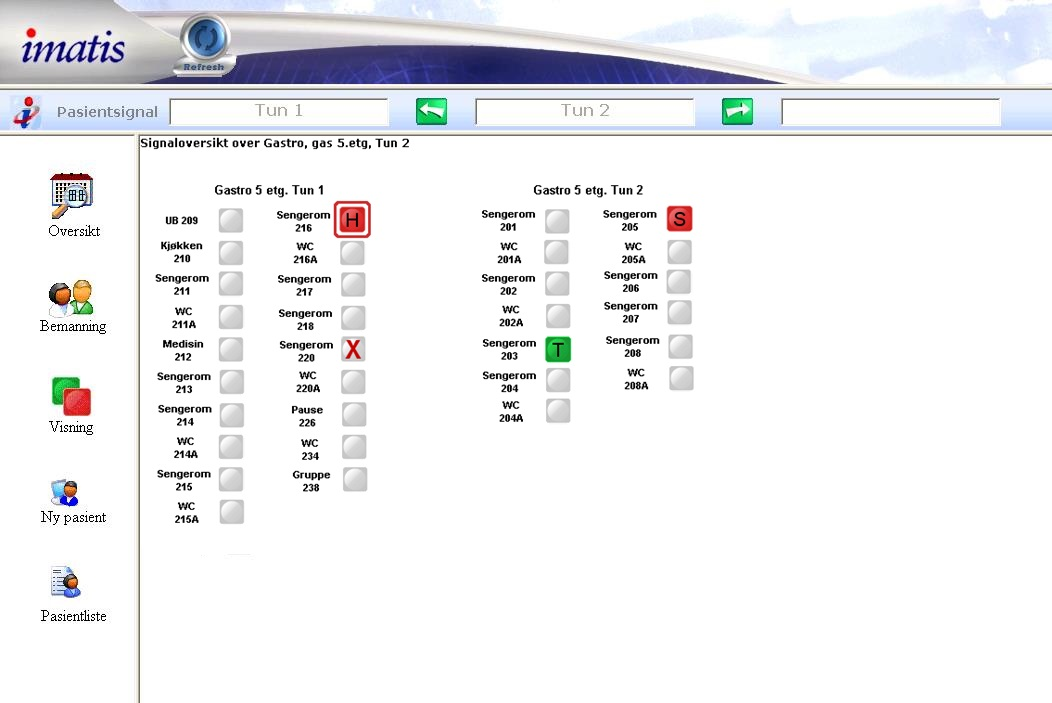
\includegraphics[scale=0.2]{pasientapplikasjon.jpg}
                \caption{Pasientsignalapplikasjon}
                \label{pasientapplikasjon}
        \end{subfigure}
        \begin{subfigure}[b]{0.35\textwidth}
        		\centering
                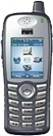
\includegraphics[scale=1]{telefon.jpg}
                \caption{Trådløs telefonenhet}
                \label{telefonenhet}
        \end{subfigure}
        \begin{subfigure}[b]{0.25\textwidth}
        		\centering
                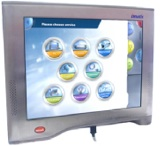
\includegraphics[scale=0.4]{pasientterminal.jpg}
                \caption{Pasientterminal}
                \label{pasientterminal}
        \end{subfigure}
        \caption{Det trådløse systemet}\label{dettradlosesystemet}
\end{figure}

\subsubsection{Pasientsignalapplikasjon}
Pasientsignalapplikasjonen kjører på en PC på hvert sengetun, 24 timer i døgnet, hver dag. Applikasjonen tilbyr i hovedsak fem funksjoner: (1) oversikt, (2) bemanning, (3) visning, (4) registrering av ny pasient og (5) en pasientliste. Vi vil her utdype funksjonene bemanning og visning, da disse er av mest relevans for vår oppgave.  

\noindent
Bemanningsplanen, vist i figur \ref{bemanningsplan}, knytter tilgjengelig pleiepersonell til rommene ved et sengetun. Pasientsignalene vil dermed sendes til riktig mottaker på bakgrunn av bemanningsplanen. For hvert rom vil det normalt tilknyttes en primærsykepleier og en disponibel sykepleier.

\begin{figure}[H]
\centering
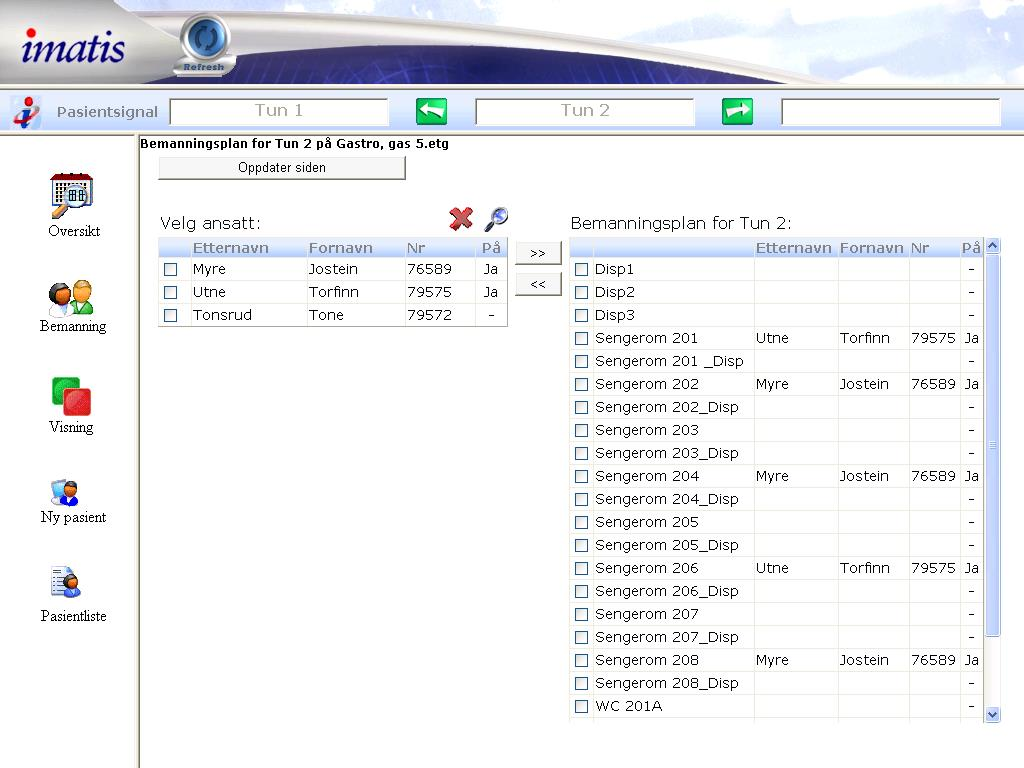
\includegraphics[scale=0.5]{bemanningsplan.jpg}
\caption{Bemanningsplan}
\label{bemanningsplan}
\end{figure}

\noindent
Funksjonen visning, vist i figur \ref{visning}, viser en oversikt over pasientsignalanlegget ved gjeldende sengetun, her vist som Gastro i 5. etasje, tun en og to. Grønn T markerer at pleiepersonell har trykket på den grønne knappen på rompanelet i det gjeldende sengerommet, og tilsynelatende er tilstede. Dette er ikke nødvendigvis riktig, da pleiepersonell kan glemme å trykke av den grønne knappen da de forlater rommet. Rød S signaliserer et pasientsignal, mens innrammet rød H signaliserer et hasteanrop. Rødt kryss varsler feil i systemet.

\begin{figure}[H]
\centering
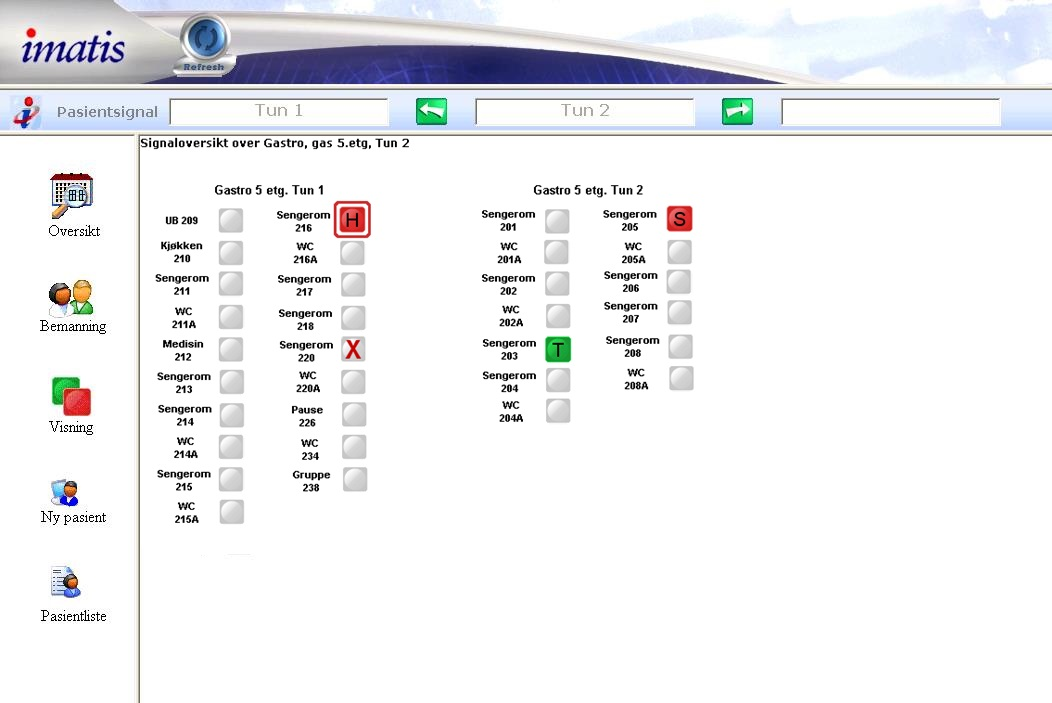
\includegraphics[scale=0.5]{pasientapplikasjon.jpg}
\caption{Visning}
\label{visning}
\end{figure}

\subsubsection{Trådløs telefonenhet}
De trådløse telefonenhetene inngår i det IP-baserte telefonisystemet ved St. Olavs Hospital, og er av typen Cisco Wireless IP Phone 7921G. I tillegg til å tilby basisfunksjoner som å ringe og sende tekstmeldinger, støtter de tjenester for alarmering. Pleiepersonell logger seg på telefonene for å motta pasientsignal og hasteanrop i forhold til ansvar gitt i bemanningsplanen.

\subsubsection{Pasientterminal}
Pasientterminalen inneholder en rekke funksjoner som pasienten kan benytte seg av, deriblant TV, radio, telefon, internett, spill og knapp for pasientsignal. Den røde knappen under skjermen benyttes for å utløse pasientsignal, og denne fungerer uavhengig av om terminalen er skrudd på eller ikke.

\pagebreak

\subsection{Hvordan det hele henger sammen}
\begin{figure}[H]
\centering
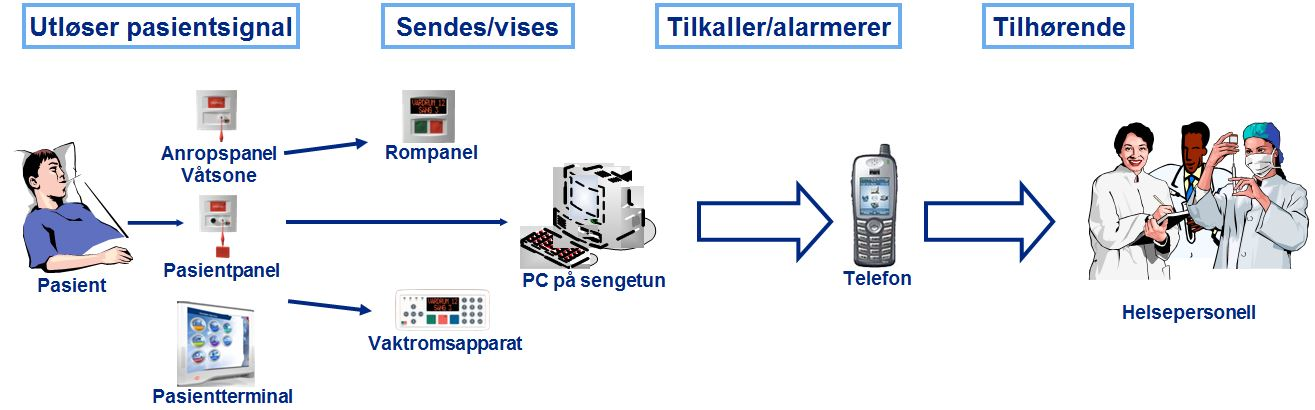
\includegraphics[scale=0.5]{alarmprosess.jpg}
\caption{Pasientsignal (Opplæring:Pasientsignal, delvis modifisert)}
\label{alarmprosess}
\end{figure}

\noindent
Pasienten kan utløse et pasientsignal ved å trykke på signalknappen på pasientterminalen, dra i snoren på anropspanelet, eller trykke på den røde knappen på rompanelet. Da vil lysdioden på rompanelet og anropspanelet blinke rødt. På andre sengerom hvor tilstedemarkering er aktivert vil lysdioden blinke rødt, og nummer- og stedsangivelse vil vises på displayet. Vaktromsapparatet vil blinke og avgi lydsignal, og pasientsignalapplikasjonen viser markering for pasientsignal.

\begin{figure}[H]
        \centering
        \begin{subfigure}[b]{0.35\textwidth}
        		\centering
                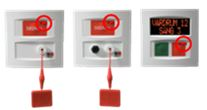
\includegraphics[scale=0.7]{signal_paneler.jpg}
        \end{subfigure}
        \begin{subfigure}[b]{0.35\textwidth}
        		\centering
                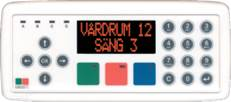
\includegraphics[scale=1]{vaktromsapparat.jpg}
                \label{telefon}
        \end{subfigure}
        \caption{Alarmering ved pasientsignal}\label{pasientsignalalarm}
\end{figure}

\begin{figure}[H]
\centering
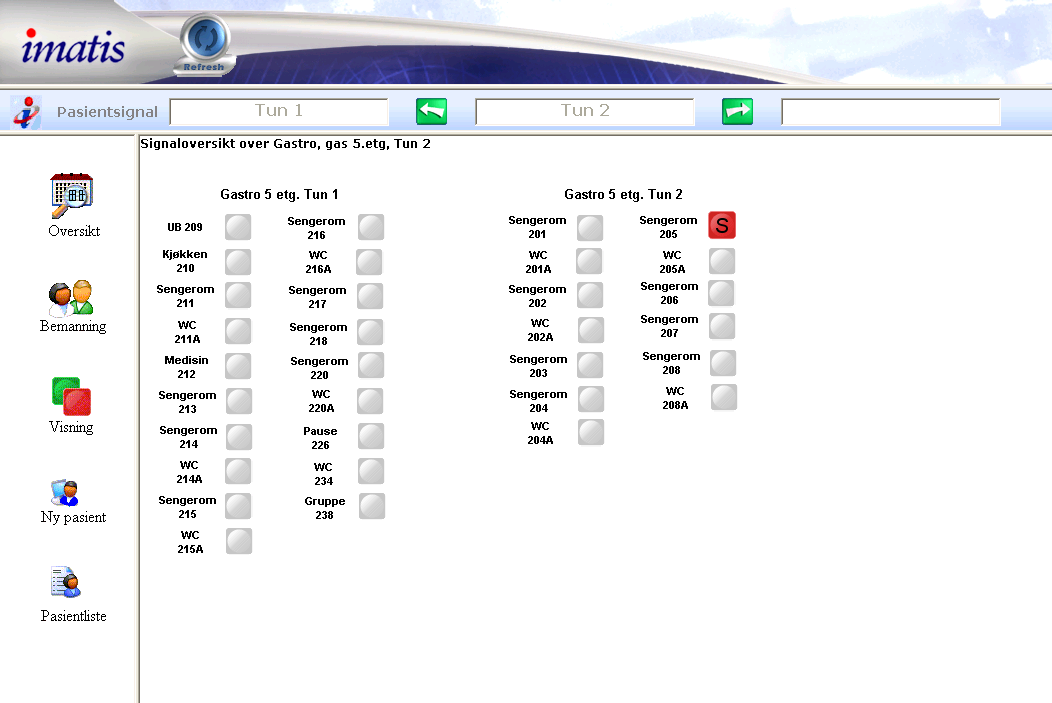
\includegraphics[scale=0.4]{applikasjonalarm.png}
\caption{Pasientsignalapplikasjon ved alarm (Brukermanual for Pasientsignal og Pasientsignalapplikasjon )}
\label{alarmprosess}
\end{figure}

\noindent
Dedikert pleiepersonell registrert i bemanningsplanen tilkalles på sin trådløse telefonenhet ved at melding vises på displayet, og lydsignal avgis. Mottaker har da mulighet til å godta eller avvise pasientsignalet. Dersom vedkommende velger å avvise tilkallingen, eller ikke foretar seg noe innen 15 sekunder, vil signalet sendes videre til neste ressurs. Slik vil det fortsette inntil tilkallingen blir bekreftet.

\begin{figure}[H]
\centering
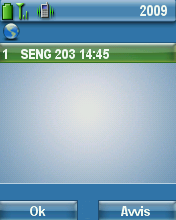
\includegraphics[scale=1]{alarmtelefon.png}
\caption{Trådløs telefonenhet ved alarm (Opplæring: Pasientsignal)}
\label{alarmprosess}
\end{figure}

\noindent
Dersom mottaker godtar tilkallingen vil den legges i mottakers arbeidsliste, og vedkommende har 2 minutter på seg for å tilstedemarkere seg på rommet, ellers vil tilkallingen videresendes til neste registrerte ressurs.

\begin{figure}[H]
\centering
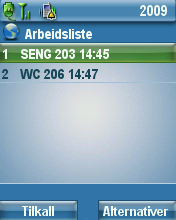
\includegraphics[scale=1]{telefonok.png}
\caption{Arbeidsliste (Opplæring: Pasientsignal)}
\label{alarmprosess}
\end{figure}

\noindent
Ved tilstedemarkering vil lyssignalet stoppe på anropspanelene, og rompanelet vil blinke med grønt lys. Vaktromsapparatet viser sengenummer og stopper lydsignalet, tilkallingen fjernes fra mottakers arbeidsliste, og pasientsignalapplikasjonen viser tilstedemarkering.
 
\begin{figure}[H]
        \centering
        \begin{subfigure}[b]{0.35\textwidth}
        		\centering
                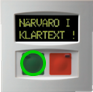
\includegraphics[scale=1]{rompanelok.png}
                \caption{Rompanel}
                \label{rompanelok}
        \end{subfigure}
        \begin{subfigure}[b]{0.25\textwidth}
        		\centering
                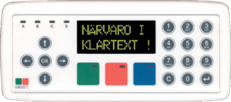
\includegraphics[scale=0.9]{vaok.png}
                \caption{Vaktromsapparat}
                \label{vaok}
        \end{subfigure}
        \caption{Det faste systemet etter tilstedemarkering}
\end{figure} 

\begin{figure}[H]
\centering
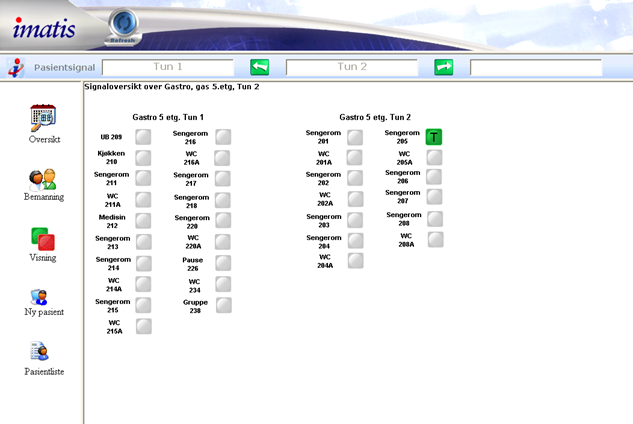
\includegraphics[scale=1]{applikasjonok.png}
\caption{Pasientsignalapplikasjon etter tilstedemarkering}
\label{applikasjonok}
\end{figure}

\noindent
Pleiepersonell trykker på den grønne knappen for å avstille pasientsignalet. Dersom pleiepersonell får behov for assistanse kan han/hun utløse et hasteanrop ved å bruke signalknappen på anropspanelet eller den røde knappen på rompanelet. Alarmen indikeres ved et hastig lydsignal, og røde tall for romnummer og stedsangivelse blinker hurtig på vaktromsapparatet og tilstedemarkerte rompaneler. På det gjeldende rommet vil både rød og grønn lysdiode blinke på rompanelet. I tillegg sendes en hasteanropsmelding, som ikke kan avvises, til samtlige av pleiepersonellets trådløse telefoner på sengetunet. Pasientsignalapplikasjonen viser markering for hasteanrop. Hasteanrop legges i arbeidsliste og avstilles på samme måte som pasientsignaler.

\begin{figure}[H]
\centering
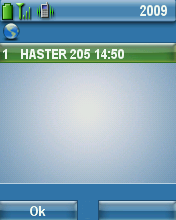
\includegraphics[scale=1]{hasteanropsmelding.png}
\caption{Trådløs telefonenhet ved hasteanrop}

\begin{figure}[H]
\centering
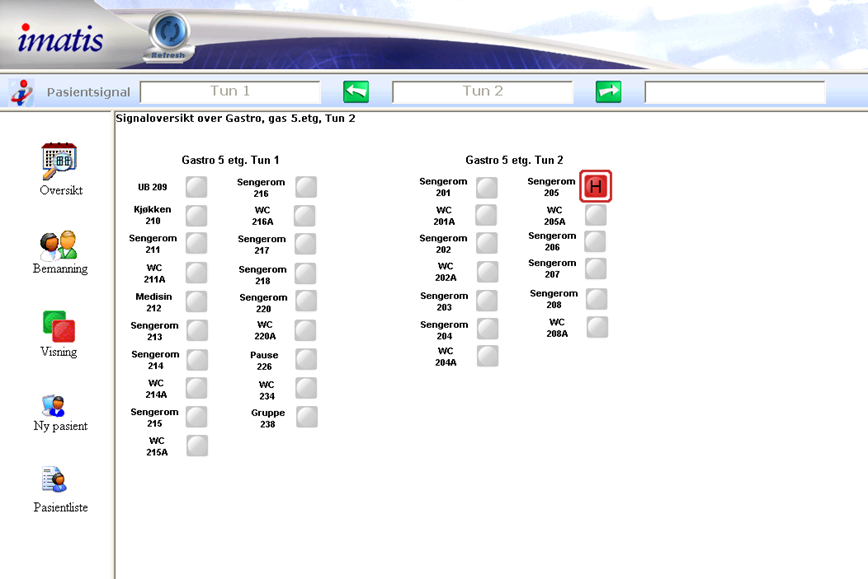
\includegraphics[scale=1]{applikasjonhast.png}
\caption{Pasientsignalapplikasjon ved hasteanrop}
\label{applikasjonok}
\end{figure}
\label{applikasjonok}
\end{figure}










